\documentclass[UTF8,a4paper,11pt]{ctexart}
\usepackage[left=2.50cm, right=2.50cm, top=2.50cm, bottom=2.50cm]{geometry} %页边距
\CTEXsetup[format={\Large\bfseries}]{section} 
 

% compile using Xelatex
%%%%%%%%%%%%%%%%%%%%%%%   字体备选栏
% -- 中文字体 --
%\setmainfont{Microsoft YaHei}  % 微软雅黑
%\setmainfont{YouYuan}  % 幼圆    
%\setmainfont{NSimSun}  % 新宋体
%\setmainfont{KaiTi}    % 楷体
%\setmainfont{SimSun}   % 宋体
%\setmainfont{SimHei}   % 黑体
% -- 英文字体 --
%\usepackage{times}
%\usepackage{mathpazo}
%\usepackage{fourier}
%\usepackage{charter}
\usepackage{helvet}
 
\usepackage{amsmath, amsfonts, amssymb} % math equations, symbols
\usepackage[english]{babel}
\usepackage{color}      % 控制文本颜色
\usepackage{graphicx}   % 加载图像包
\usepackage{url}        % 网址超链接
\usepackage{bm}         % equations的粗体形式
\usepackage{tikz}       % tikz 图像包
\usepackage{multirow}	% 列表设置一格多行多列
\usepackage{ulem}
\usepackage{booktabs}
\usepackage{epstopdf}
\usepackage{epsfig}
\usepackage{algorithm}  %编写算法

\usepackage{hyperref} %此处设置文本内超链接

%\usepackage{CJK,pgf,pgfarrows,pgfnodes,pgfautomata,pgfheaps}
\usepackage{amsmath,amssymb}
\usepackage{geometry}%页面设置
\usepackage{graphicx}%图片设置
\usepackage{float} %指定图片位置
%\usepackage{subfig}%多个子图
\usepackage{subfigure}%并排子图 共享标题 有子标题
\usepackage{caption}%注释设置

\usepackage{algorithm}
\usepackage{algorithmicx}
\usepackage{algpseudocode}  

% 这个和algorithmic不兼容,用了就要报错,好多莫名其妙的错误!!!!!
\floatname{algorithm}{算法}  
\renewcommand{\algorithmicrequire}{\textbf{输入:}}  
\renewcommand{\algorithmicensure}{\textbf{输出:}}  
\renewcommand{\algorithmicrequire}{ \textbf{Input:}}     %Use Input in the format of Algorithm
\renewcommand{\algorithmicensure}{ \textbf{Output:}}    %UseOutput in the format of Algorithm

\newtheorem{pf}{Pf}
\newtheorem{sol}{Sol}[section]
\newtheorem{thm}{Thm}
\newtheorem{ex}{e.g.}
% 算法示例备选项
%\renewcommand{\algorithmicrequire}{ \textbf{Input:}}     % use Input in the format of Algorithm  
%\renewcommand{\algorithmicensure}{ \textbf{Initialize:}} % use Initialize in the format of Algorithm  
%\renewcommand{\algorithmicreturn}{ \textbf{Output:}}     % use Output in the format of Algorithm  

\DeclareMathOperator{\dif}{d\!}  %定义微分的缩写
\DeclareMathOperator{\pa}{\partial}  %定义偏微分的缩写

%\usepackage{fancyhdr}  %这里对 页眉、页脚 进行设置
%\pagestyle{fancy}
%\rhead{\thepage}
%\chead{}
%%\lhead{\includegraphics[width=1.6cm]{wallpaper.jpg}}
%\lfoot{}
%\cfoot{Page \thepage{} of \pageref{LastPage}}
%\rfoot{}
%
%\newcommand{\makeheadrule}{%        %去除页眉的横线 以免遮挡后面文字 
%	\makebox[0pt][l]{\rule[0\baselineskip]{\headwidth}{0pt}}%
%	\rule[0\baselineskip]{\headwidth}{0pt}}
%\renewcommand{\headrule}{%
%	{\if@fancyplain\let\headrulewidth\plainheadrulewidth\fi
%		\makeheadrule}}

%\usepackage[printwatermark]{xwatermark}   %%这以下设置“数学外卖”官方水印
%\usepackage{lipsum}
%
%\newsavebox\mybox
%
%\savebox\mybox{\tikz[color=gray,opacity=0.3]
%\newwatermark*[
%allpages,
%angle=48,
%scale=6,
%xpos=-20,
%ypos=15
%]{\usebox\mybox} 
 


\title{\textbf{Homework 2}}
\author{ 张思源  \qquad  \textit{21110850018} }   %这里填上您的大名


\begin{document}
\maketitle
\section{Ex1}
\par 在导入mnist数据集后,首先对数据集进行可视化,只需要对DataFrame格式的图片矩阵化,然后进行reshape即可,具体结果如下图所示:
\begin{figure}[H]
	\centering
	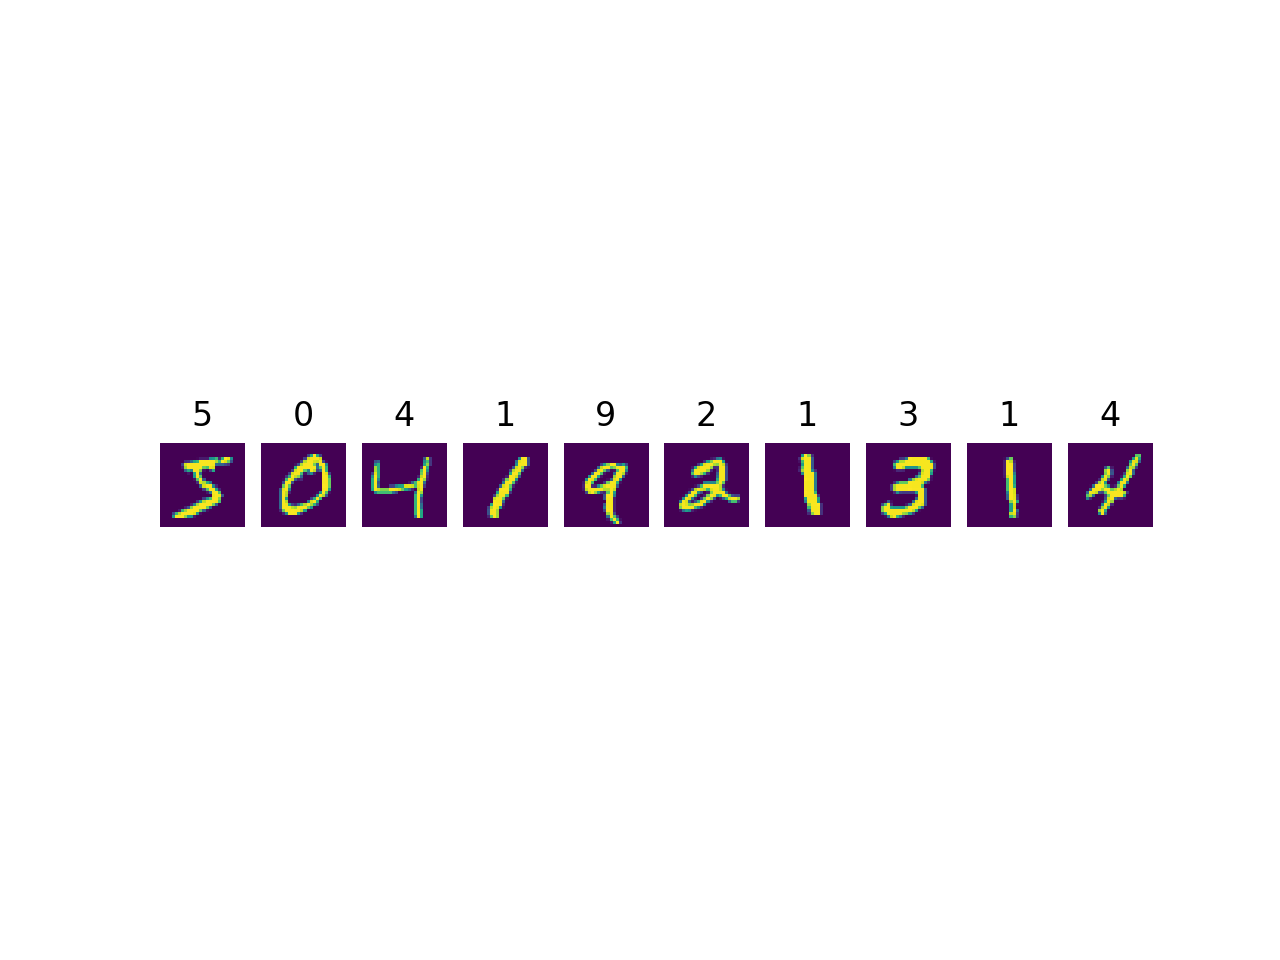
\includegraphics[width=0.5\textwidth,height=0.5\textwidth]{show.png}
	\caption{Some examples of mnist}
\end{figure}
\par 之后,对各个标签(即数字0到9)对应的向量化图像的数目进行统计,以判断是否存在数据差异过大的情况,因为在数据差异过大的情况下直接对数据进行分类操作易出现问题.经过统计,\textbf{各个标签对应的向量化图像的数目差距不大,且由于数据维数较高(784维),数据的凸包几乎不可能不相交,故数据是线性不可分的,这是mnist数据集最重要的特点}.
具体如下图所示:
\begin{figure}[H]
	\centering
	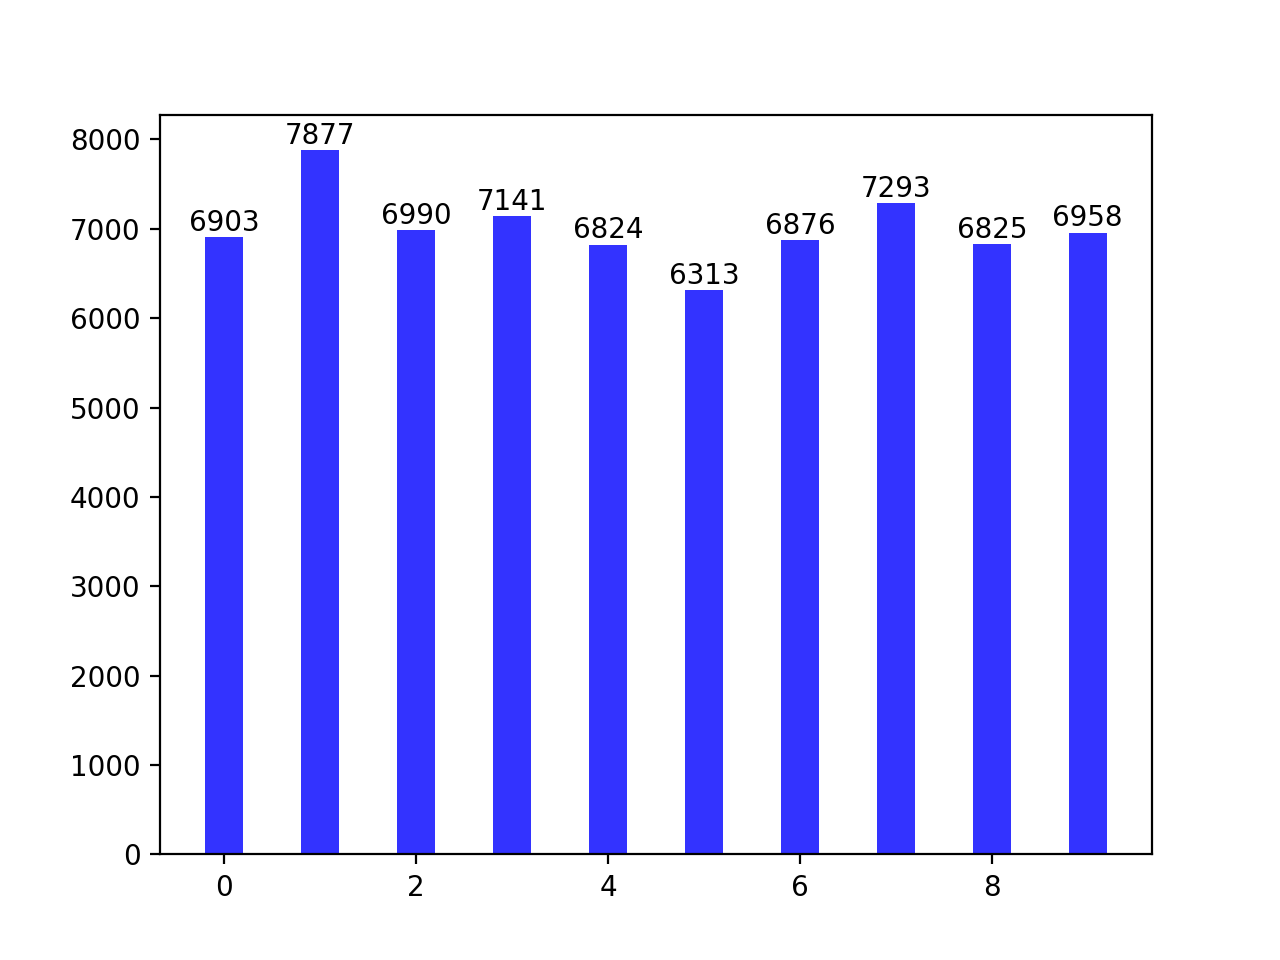
\includegraphics[width=0.7\textwidth,height=0.5\textwidth]{figure.png}
	\caption{Number of data corresponding to different labels}
\end{figure}
为了更好说明这一步工作的重要性,这里引入一个特殊的例子:
\begin{ex}
	考虑同一个数据集即mnisit数据集,这时任务考虑为二分类任务,即区分对于一个手写数字,是0还是非0.不妨假设0到9各个数字对应的图像数目是相等的,此时我们训练分类器的方法为无论标签为哪个数字,对应的输出结果均为非0,这样我们得到的结果准确率可达90\%,但是召回率会非常低,这说明当不同类规模差距较大时,我们需要对其进行预处理.
\end{ex}
\par 在此基础上,利用留出法,划出70000个数据中的后10000个数据为测试集,其余数据为训练集,选取kernel为rbf,即高斯核函数,去训练模型,并记录模型的训练与测试时间,在2.6 GHz 六核Intel Core i7的cpu,python3.8下训练时间和 测试时间如下图所示:
\begin{figure}[H]
	\centering
	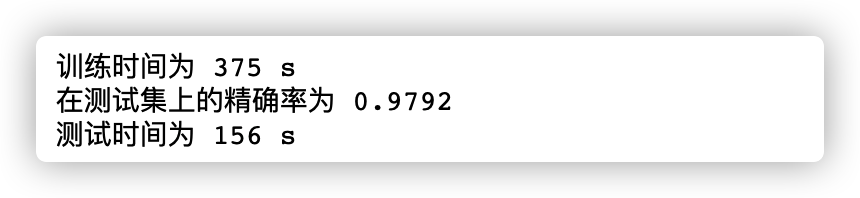
\includegraphics[width=1.0\textwidth,height=0.2\textwidth]{SVM_result.png}
	\caption{Results of SVM}
\end{figure}
\par 最终模型在测试集上的准确率为0.9792,可以看出模型较好的对10种手写数字图像进行了分类.同时模型的混淆矩阵如下图,可以看出模型同时有着较高的召回率和精确率.
\begin{figure}[H]
	\centering
	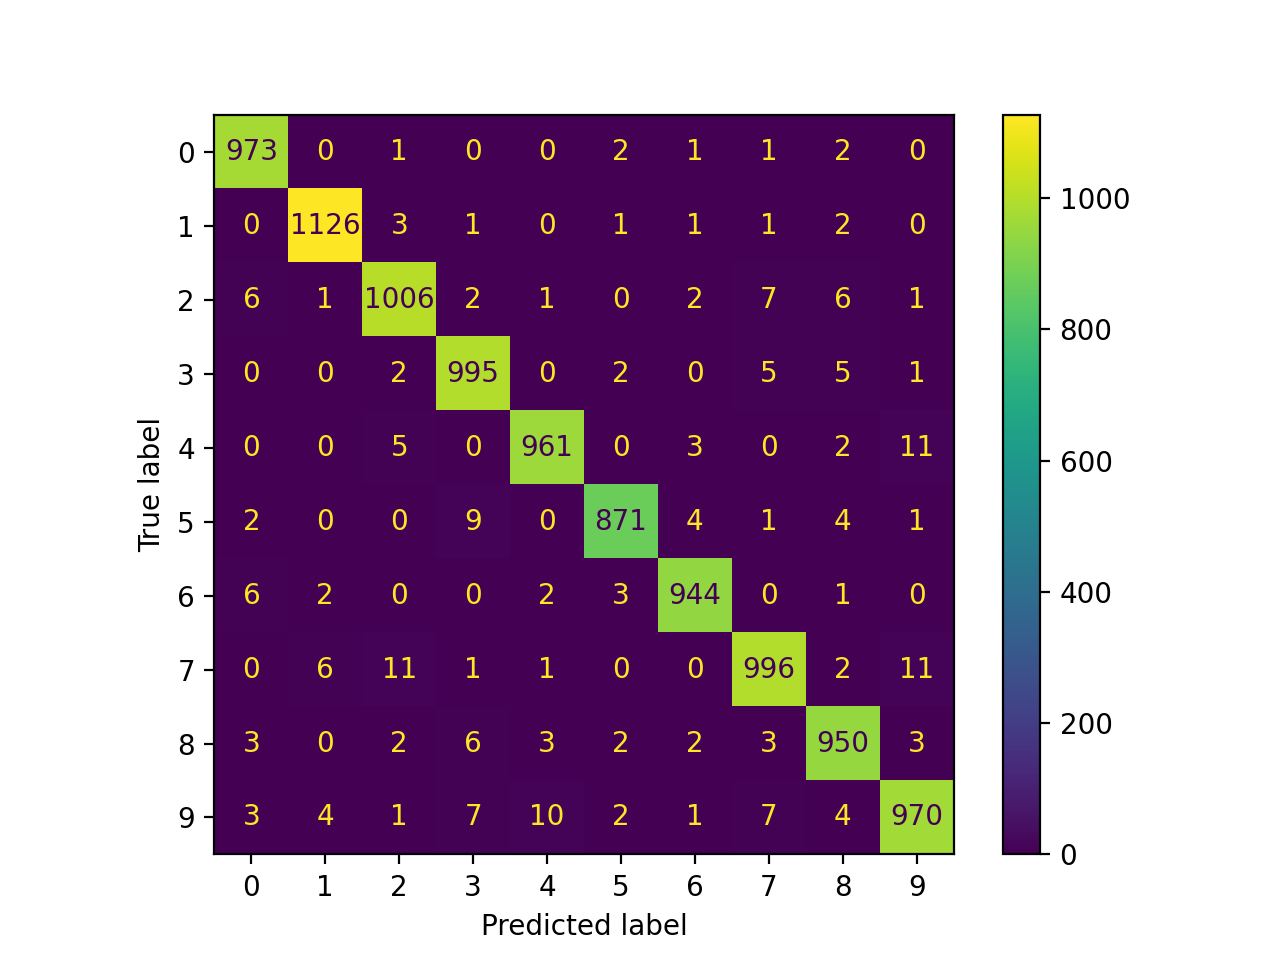
\includegraphics[width=0.7\textwidth,height=0.5\textwidth]{cm.png}
	\caption{Confusion matrix}
\end{figure}

而对于全连接网络,这里使用了pytorch构建全连接网络,网络结构为5层,具体结构如下图所示:
\begin{figure}[H]
	\centering
	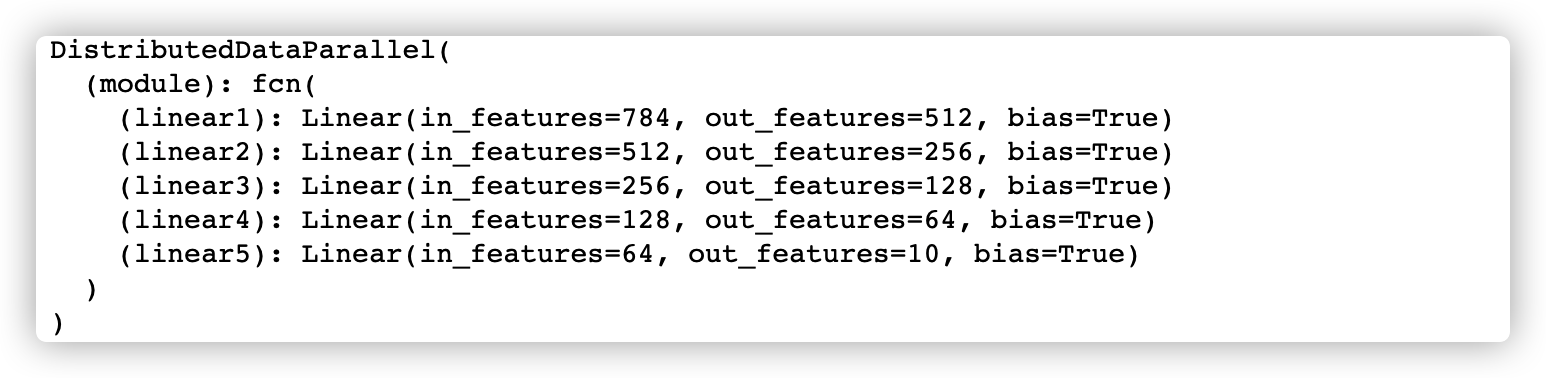
\includegraphics[width=\textwidth,height=0.5\textwidth]{net.png}
	\caption{Fully connected network}
\end{figure}
进而执行训练与测试,可以得到训练时间与测试精确率如下图所示:
\begin{figure}[H]
	\centering
	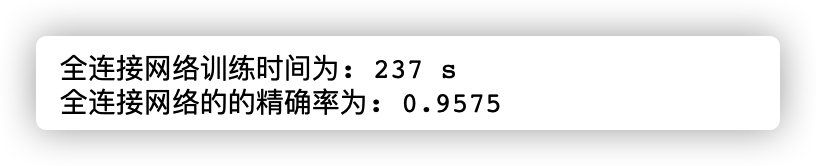
\includegraphics[width=\textwidth,height=0.2\textwidth]{FC_result.png}
	\caption{Results of fully connected network}
\end{figure}
可以看出,SVM方法与全连接网络方法的精确率差距不大,但是由于全连接网络可以调用服务器计算,
这里调用的类脑集群服务器GPU15节点GTX1080Ti*3,可以大大提高计算效率.
\newpage
\begin{thebibliography}{3}  
	\bibitem{ref1} 李航. 统计学习方法[M]. 清华大学出版社, 2012.
	%\bibitem{ref2} Kingma D , Ba J . Adam: A Method for Stochastic Optimization[J]. Computer Science, %2014.
	\bibitem{ref2} Goodfellow, Ian, et al. Deep Learning[M]. MIT Press, 2016. 	
	\bibitem{ref3} Peter Harrington, 李锐 … [等. 机器学习实战[M]. 人民邮电出版社, 2013.
\end{thebibliography}
\end{document}
